\documentclass[a4paper]{book} %{article}

\usepackage{fullpage} % Package to use full page
\usepackage{parskip} % Package to tweak paragraph skipping
\usepackage{tikz} % Package for drawing
\usepackage{amsmath}
\usepackage{hyperref}
\usepackage[numbered]{bookmark} % For numbering of challenges in bookmark pane of PDF viewer
\def\UrlBreaks{\do\/\do-}
\usepackage[absolute]{textpos}
\setlength{\TPHorizModule}{1mm}
\setlength{\TPVertModule}{1mm}
\usepackage{tikz}
\usepackage{siunitx}
\usepackage{datetime} % Time
\usepackage[UKenglish]{isodate}
\usepackage{ctable} % Thick table lines
\usepackage{booktabs} % Merge cells with multicolumn

\newcommand{\disctime}{10:30 to 12:00 }
\newcommand{\discdays}{Fridays }
\newcommand{\discroom}{W4-529}
\newcommand{\discexam}{10th February 2017}
\newcommand{\course}{Ordinary Differential Equations }
\newcommand{\courseurl}{ordinary-differential-equations}
\newcommand{\nensei}{2nd}
\newcommand{\assstart}{21 October}

\newcommand{\six}[1]{\SI[parse-numbers=false]{X}{#1}}
\newcommand{\hash}[2]{MD5(#1\_X) = #2\ldots}
\newcommand{\timebox}{\vfill Study-time (from end of previous challenge to end of this challenge): \underline{\hspace{1cm} minutes}}

\graphicspath{{Images/}}

\begin{document}

\begin{titlepage}
    \begin{center}
        \vspace*{1cm}

        \Huge
        \textbf{Ordinary Differential Equations}

        Autumn 2016

        \vspace{1.5cm}
        \Large
        Last updated:\\\today \ at \currenttime

        \vspace{4.0cm}
        \LARGE
        James Cannon\\Kyushu University
        \vfill

        \normalsize
        \url{http://www.jamescannon.net/teaching/\courseurl}\\
        \vspace{0.3cm}
        \small
        \url{http://raw.githubusercontent.com/NanoScaleDesign/OrdinaryDifferentialEquations/master/ode.pdf}
        \vspace{0.5cm}

        License: \emph{CC BY-NC 4.0}.

    \end{center}
\end{titlepage}

\setcounter{chapter}{-1}

\tableofcontents

\chapter{Course information}
\newpage
\section{This course}
This course is the \course course studied at Kyushu University by \nensei-year students.

\subsection{How this works}
\begin{itemize}
    \item In contrast to the traditional lecture-homework model, in this course the learning is self-directed and active via publicly-available resources.
    \item Learning is guided through solving a series of carefully-developed challenges contained in this book (download from \url{http://www.jamescannon.net/teaching/\courseurl}), coupled with suggested resources that can be used to solve the challenges with instant feedback about the correctness of your answer.
    \item There are no lectures. Instead, there is discussion time. Here, you are encouraged to discuss any issues with your peers, teacher and any teaching assistants. Furthermore, you are encouraged to help your peers who are having trouble understanding something that you have understood; by doing so you actually increase your own understanding too.
    \item Peer discussion is encouraged, however, if you have help to solve a challenge, always make sure you do understand the details yourself. You will need to be able to do this in an exam environment. If you need additional challenges to solidify your understanding, then ask the teacher. The questions on the exam will be similar in nature to the challenges. If you can do all of the challenges, you can get 100\% on the exam.
    \item Discussion-time is from \disctime on \discdays at room \discroom.
    \item Every challenge in the book typically contains a \textbf{Challenge} with suggested \textbf{Resources} which you are recommended to utilise in order to solve the challenge. A \textbf{Solution} is made available in encrypted form. If your encrypted solution matches the encrypted solution given, then you know you have the correct answer and can move on. For more information about encryption, see section \ref{sec:hashes}. Occasionally the teacher will provide extra \textbf{Comments} to help guide your thinking.
    \item For deep understanding, it is recommended to study the suggested resources beyond the minimum required to complete the challenge.
    \item The challenge document has many pages and is continuously being developed. Therefore it is advised to view the document on an electronic device rather than print it. The date on the front page denotes the version of the document. You will be notified by email when the document is updated.
    \item A “target challenge” and “minimum challenge” will be set each week, to be achieved by the beginning of the discussion time.
    \begin{itemize}
        \item Target challenge: You are expected to complete at least up to this challenge. This is because the “group learning” effect is strongest when everyone is roughly around the same level of understanding.
        \item Minimum challenge: Due to personal (eg health) or professional (eg conference attendance) issues, or simply difficulties with the challenges, it may occasionally not be possible to reach the target challenge. In this case, you will still be considered to be progressing normally if you achieve the minimum challenge.
        \item You may work ahead, even beyond the target challenge, if you so wish. This can build greater flexibility into your personal schedule, especially as you become busier towards the end of the semester.
    \end{itemize}
    \item Your contributions to the course are strongly welcomed. If you come across resources that you found useful that were not listed by the teacher or points of friction that made solving a challenge difficult (there's no such thing as ``you should have learned it in high-school'' - you're probably not the only one with that specific problem), please let the teacher know about it!
\end{itemize}

\subsection{Assessment}
In order to prove to outside parties that you have learned something from the course, we must perform summative assessments. This will be in the form of
\begin{itemize}
    \item Exam(s): Final exam, and possibly a mid-term exam
    \item Group presentation towards the end of the course (details to be announced later)
\end{itemize}

\subsection{What you need to do}
\begin{itemize}
    \item Prepare a challenge-log in the form of a workbook or folder where you can clearly write the calculations you perform to solve each challenge. This will be a log of your progress during the course and will be occasionally reviewed by the teacher.
    \item You will need to maintain a google spreadsheet detailing your work and progress. The purpose of this spreadsheet is to help the teacher optimise the discussion-time. Please ensure that it is up-to-date 24 hours before each discussion-time starts. It is fine for you to continue to work on challenges and update the spreadsheet after the 24-hour deadline.
    \item You also need to submit a brief report at \url{https://goo.gl/forms/Djl4FEZcJLMpipsY2} 24 hours before the discussion time starts. Here you can let the teacher know about any difficulties you are having and if you would like to discuss anything in particular.
    \item Please bring a wifi-capable internet device to class, as well as headphones if you need to access online components of the course during class. If you let me know in advance, I can lend computers and provide power extension cables for those who require them (limited number).
\end{itemize}

\subsection{Details about the spreadsheet}
To get started:
\begin{enumerate}
    \item Log into google
    \item Open \url{http://bit.ly/2cPYyQY}
    \item File $\rightarrow$ Make a copy [$\rightarrow$ rename] $\rightarrow$ ok
    \item Click ``Share'' (top right)
    \item Click ``Get shareable link''
    \item Set ``Anyone with the link can view''
    \item Copy sharing address
    \item Send an email to cannon@mech.kyushu-u.ac.jp containing
    \begin{enumerate}
       \item Subject: [course name] registration
       \item Your name
       \item Student number
       \item The link to your copy of the google sheet
    \end{enumerate}
\end{enumerate}

Using the spreadsheet:

\begin{itemize}
    \item Enter the appropriate challenge number. For example, for challenge 1.4, enter ``1'' in the \textbf{Section} column and ``4'' in the \textbf{Challenge} column.
    \item After successfully completing a challenge, please enter any particular friction points that you experienced (if any) so the course can be developed to reduce such friction in the future, as well as any extra resources you recommend (if any).
    \item Please also roughly estimate the amount of effort in \textbf{Hours} required to complete the challenge (starting from when you completed the previous challenge, including any reading, watching videos, looking for resources, writing the answer to the challenge, discussing with peers, etc). This is not used for assessment in any way, but is very valuable in helping the teacher develop the course.
\end{itemize}

Note: Please do not alter column names, ordering, etc. Just add section and challenge numbering and fill in the columns as appropriate. This is because spreadsheet data is downloaded and automatically analysed, and it breaks if anything is inconsistent.



\newpage
\section{Timetable}

\begin{center}
    \begin{tabular}{|c|c|c|c|}
        \hline
        & \textbf{Discussion} & \textbf{Target} & \textbf{Note} \\ \specialrule{.1em}{.05em}{.05em}
        \textbf{1}  & 7 Oct  & -            &                          \\ \hline
        \textbf{2}  & 14 Oct & 2.2          &                          \\ \hline
        \textbf{3}  & 21 Oct & 2.7          &                          \\ \hline
        \textbf{4}  & 28 Oct & 2.12         &                          \\ \specialrule{.1em}{.05em}{.05em}
        \textbf{5}  & 4 Nov  & 2.20         &                          \\ \hline
        \textbf{6}  & 11 Nov & 3.8          &                          \\ \hline
        \textbf{7}  & 25 Nov & 3.15         &                          \\ \specialrule{.1em}{.05em}{.05em}
        \textbf{8}  & 2 Dec  & 3.18         & Coursework instructions  \\ \hline                            % Non-homogeneous equations (undetermined coeffs, var of params)
        \textbf{9}  & 9 Dec  & Midterm exam &                          \\ \hline                            % Exam preparation
        \textbf{10} & 16 Dec & 4.6          &                          \\ \specialrule{.1em}{.05em}{.05em}  % Laplace transform
        \textbf{11} & 6 Jan  & 4.12         &                          \\ \hline                            % Laplace transform
        \textbf{12} & 12 Jan & 5.3          & Submission of coursework \\ \hline                            % Systems of differential equations
        \textbf{13} & 20 Jan &              &                          \\ \hline                            % Systems of differential equations
        \textbf{14} & 27 Jan &              &                          \\ \specialrule{.1em}{.05em}{.05em}  % Series
        \textbf{15} & 10 Feb & Final exam   & Open learning plaza room 4 \\ \hline
    \end{tabular}
\end{center}

Example: To keep pace with the course, you should aim to complete challenge 2 of chapter 2 by the 14th of October.

\newpage
\section{Hash-generation}
\label{sec:hashes}

Most solutions to challenges are encrypted using MD5 hashes. In order to check your solution, you need to generate its MD5 hash and compare it to that provided.  MD5 hashes can be generated at the following sites:

\begin{itemize}
    \item Wolfram alpha: (For example: md5 hash of ``q\_1.00'') \url{http://www.wolframalpha.com/input/?i=md5+hash+of+\%22q_1.00\%22}
    \item \url{www.md5hashgenerator.com}
\end{itemize}

Since MD5 hashes are very sensitive to even single-digit variation, you must enter the solution exactly. This means maintaining a sufficient level of accuracy when developing your solution, and then entering the solution according to the format below:

Unless specified otherwise, any number from $0.00$ to $\pm 9999.99$ should be represented as a normal number to two decimal places. All other numbers should be in scientific form. See the table below for examples.

\begin{center}
\begin{tabular}{|l|l|}
    \hline
    \textbf{Solution} & \textbf{Input} \\ \hline
    1 & 1.00 \\
    -3 & -3.00 \\
    -3.5697 & -3.57 \\
    0.05 & 0.05 \\
    0.005 & 5.00e-3 \\
    50 & 50.00 \\
    500 & 500.00 \\
    5000 & 5000.00 \\
    50,000 & 5.00e4 \\
    $5 \times 10^{-476}$ & 5.00e-476 \\
    $5.0009 \times 10^{-476}$ & 5.00e-476 \\
    $-\infty$ & -infinity (never ``infinite'')\\
    $2 \pi$ & $6.28$ \\
    i & im(1.00) \\
    2i & im(2.00) \\
    1 + 2i & re(1.00)im(2.00) \\
    -0.0002548 i & im(-2.55e-4) \\
    1/i = i/-1 = -i & im(-1.00) \\
    $e^{i2\pi}$ [$= cos(2 \pi) + isin(2 \pi) = 1 + i0 = 1$] & 1.00 \\
    $e^{i\pi/3}$ [$= cos(\pi/3) + isin(\pi/3) = 0.5 + i 0.87$] & re(0.50)im(0.87) \\
    Choices in order A, B, C, D & abcd \\
    \hline
\end{tabular}
\end{center}

Entry format is given with the problem. So ``q\_X'' means to enter ``q\_X'' replacing ``X'' with your solution. The first 6 digits of the MD5 sum should match the given solution (MD5(q\_X)= \ldots).

Note that although some answers can usually only be integers (eg, number of elephants), for consistency, to generate the correct hash, the accuracy in terms of decimal places noted above is required.


\chapter{Definitions}
\section{Order of a differential equation}

\subsection*{Resources}
\begin{itemize}
    \item Text: \url{http://tutorial.math.lamar.edu/Classes/DE/Definitions.aspx}
\end{itemize}

\subsection*{Challenge}
What is the sum of the orders of the following equations?

\begin{equation}
    \frac{dy}{dx}A = 5x^3 + 3
\end{equation}

\begin{equation}
    cos(y) y'''(x) - y(x) = 25
\end{equation}

\begin{equation}
    \frac{d}{dx} \frac{d^2 y}{dx^2} = \frac{x^{-2}}{3}
\end{equation}

\subsection*{Solution}
\six{}

\hash{e}{adb5a9}

\timebox


%%%%%%%%%%%%%%%%%%%%%%%%%%%%%%%%%
\newpage
%%%%%%%%%%%%%%%%%%%%%%%%%%%%%%%%%

\section{Linear equations}

\subsection*{Resources}
\begin{itemize}
    \item Text: \url{http://tutorial.math.lamar.edu/Classes/DE/Definitions.aspx}
\end{itemize}

\subsection*{Challenge}
Sum the points corresponding to the equations that are linear:

1 point: $\frac{dy}{dx} = 5x^3 + 3$.

2 points: $cos(y) y'''(x) - y(x) = 25$.

4 points: $\frac{d}{dx} \frac{d^2 y}{dx^2} = \frac{x^{-2}}{3}$.

8 points: $y'(x) - sin(y(x)) = 0$.

16 points: $y'(x) - y(x) = 0$.

32 points: $x y'(x) - y(x) = 0$.

\subsection*{Solution}
\six{}

\hash{r}{9aea7d}

\timebox


%%%%%%%%%%%%%%%%%%%%%%%%%%%%%%%%%
\newpage
%%%%%%%%%%%%%%%%%%%%%%%%%%%%%%%%%

\section{Valid solutions}

\subsection*{Resources}
\begin{itemize}
    \item Text: \url{http://tutorial.math.lamar.edu/Classes/DE/Definitions.aspx}
\end{itemize}

\subsection*{Challenge}

Use substitution to prove that

\begin{equation}
    y=\frac{5}{5+x}
\end{equation}

is a solution to the equation

\begin{equation}
    x y'+y=y^2
\end{equation}

and state the value of $x$ for which the solution is undefined.

\subsection*{Solution}
Value of $x$ for which solution is undefined: \six{}

\hash{t}{c69a20}

\timebox


%%%%%%%%%%%%%%%%%%%%%%%%%%%%%%%%%
\newpage
%%%%%%%%%%%%%%%%%%%%%%%%%%%%%%%%%

\section{Range of valid solutions}

\subsection*{Resources}
\begin{itemize}
    \item Text: \url{http://tutorial.math.lamar.edu/Classes/DE/Definitions.aspx}
\end{itemize}

\subsection*{Challenge}

Use substitution to prove that

\begin{equation}
    y = -\sqrt{100-x^2}
\end{equation}

is a solution to the equation

\begin{equation}
    x + y y' = 0
\end{equation}

and state the range of x for which the solution is valid. Enter the value of the lower range as the solution below.

\subsection*{Solution}
\six{}

\hash{y}{ef0eb9}

\timebox

% In addition, cover initial conditions
\chapter{1st-order differential equations}
\section{Determining a simple DE from a description}
% NT: Add Khan example and then do a different but similar-style problem.

\subsection*{Resources}
\begin{itemize}
    \item Text: \url{http://tutorial.math.lamar.edu/Classes/DE/Definitions.aspx}
\end{itemize}

\subsection*{Challenge}
Newton's law of cooling states that the rate of cooling of an object is proportional to the temperature difference with the ambient surroundings. (a) Write a differential equation describing this situation. (b) Assuming a proportionality constant of \num{0.2} \si{/hour}, what is the rate of temperature change when the object is at \SI{30}{\degreeCelsius} and the ambient temperature is \SI{20}{\degreeCelsius}?

\subsection*{Solution}
(units: \si{\degreeCelsius\per\hour})

\soltwodp{q}{4aca8d}




%%%%%%%%%%%%%%%%%%%%%%%%%%%%%%%%%
\newpage
%%%%%%%%%%%%%%%%%%%%%%%%%%%%%%%%%
\section{Direction (Slope) fields}

\subsection*{Resources}
\begin{itemize}
    \item Text: \url{http://tutorial.math.lamar.edu/Classes/DE/DirectionFields.aspx}
    \item Video 1: \url{https://www.khanacademy.org/math/differential-equations/first-order-differential-equations/differential-equations-intro/v/creating-a-slope-field}
    \item Video 2: \url{https://www.khanacademy.org/math/differential-equations/first-order-differential-equations/differential-equations-intro/v/slope-field-to-visualize-solutions}
\end{itemize}

\subsection*{Comment}
It is good practise to try drawing the below fields before looking at the next page. You need to be able to go in both directions (ie, drawing and recognising). You will not be given a glimps at the fields in the exam prior to being asked to draw them.

\subsection*{Question}
Try drawing the slope field for at least 3 of the equations given below (your choice). Then, put the slope fields given on the next page in the same order as these equations.

\begin{enumerate}
    \item $y'=x$
    \item $y'=0.2y$
    \item $y'=0.2y(1-y/6)$
    \item $y'=(x-y)/(x+y)$
    \item $y'=2(y-1)/x$
    \item $y'=2y/(x+5)$
\end{enumerate}

\newpage

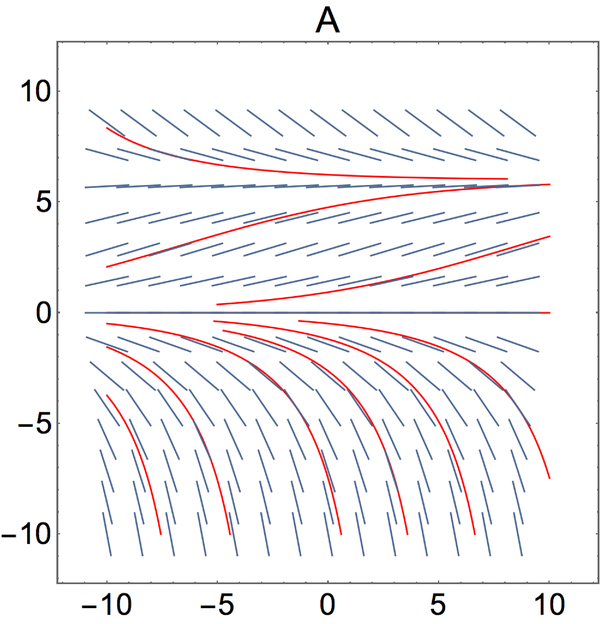
\includegraphics{direction_fields_A.png}
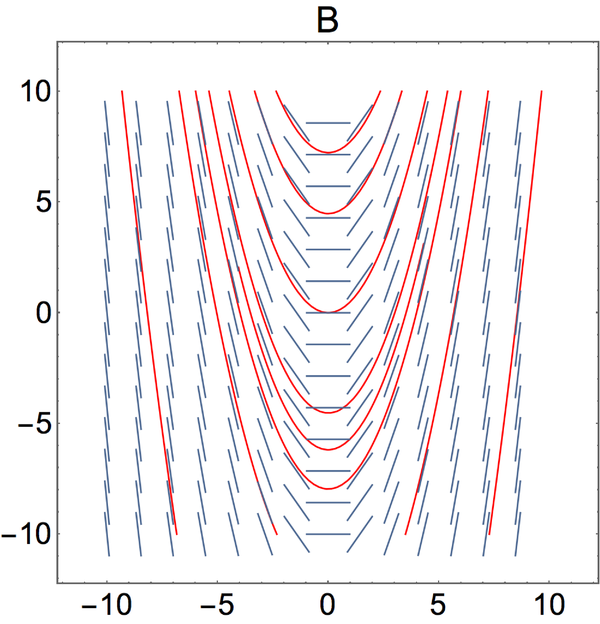
\includegraphics{direction_fields_B.png}
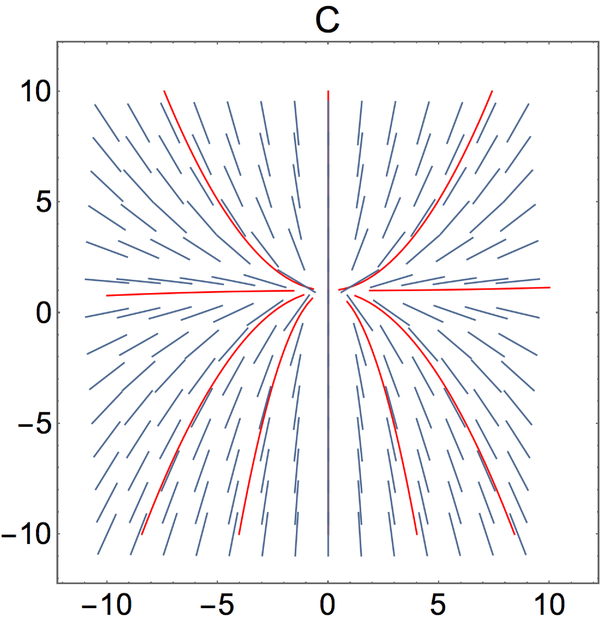
\includegraphics{direction_fields_C.png}

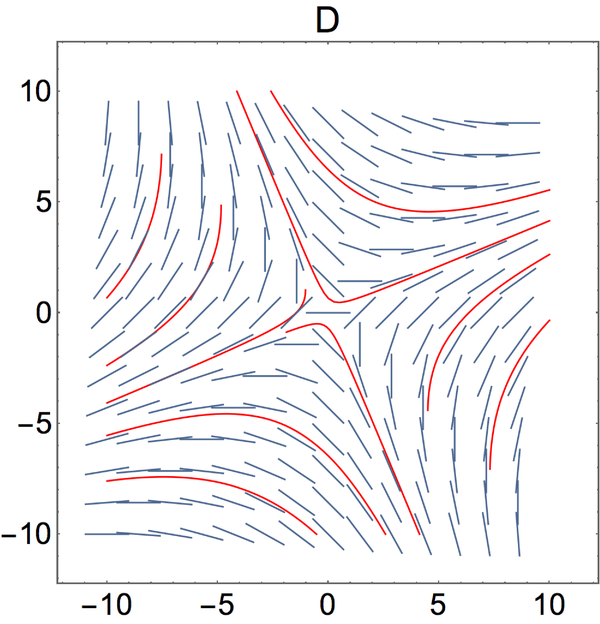
\includegraphics{direction_fields_D.png}
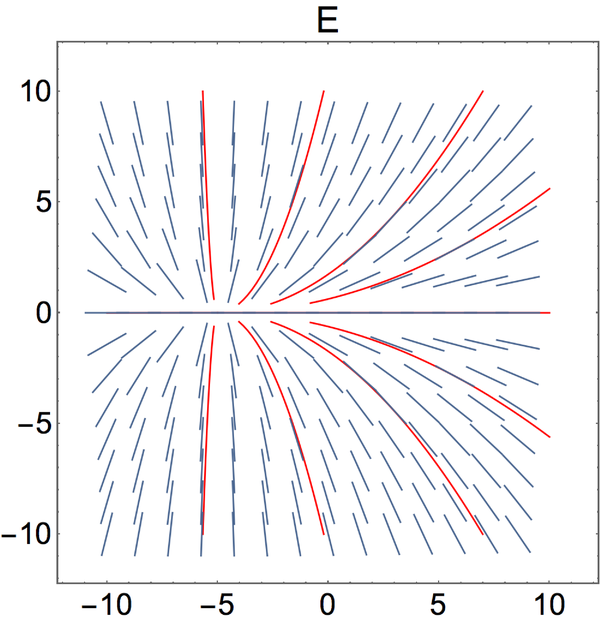
\includegraphics{direction_fields_E.png}
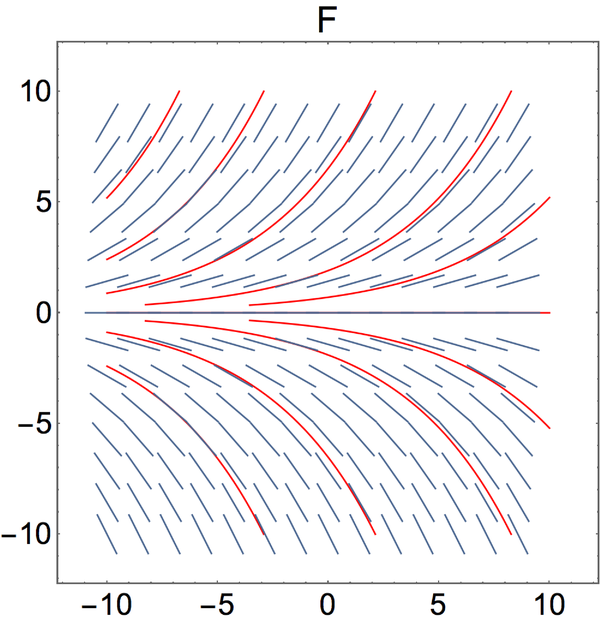
\includegraphics{direction_fields_F.png}

\subsection*{Solution}
\solstr{q}{e93bfe}



%%%%%%%%%%%%%%%%%%%%%%%%%%%%%%%%%
\newpage
%%%%%%%%%%%%%%%%%%%%%%%%%%%%%%%%%
\section{Separable equations I}
\label{sec:sepy}

\subsection*{Resources}
\begin{itemize}
    \item Video I: \url{https://www.khanacademy.org/math/differential-equations/first-order-differential-equations/separable-equations/v/separable-differential-equations-introduction} 
    \item Video II: \url{https://www.khanacademy.org/math/differential-equations/first-order-differential-equations/separable-equations/v/particular-solution-to-differential-equation-example}
    \item Text:\url{http://tutorial.math.lamar.edu/Classes/DE/Separable.aspx}
\end{itemize}

\subsection*{Comment}
Let's start with a fundamental equation:
\begin{equation}
    \frac{dy}{dt} = y
\end{equation}
This is saying that the slope (the rate of change of y) linearly depends on $y$. That is, that as the value of y increases, the slope also increases; a positive feedback loop. In fact, you get an exponentially-increasing function.

So one aim of this course is to be able to solve such equations mathematically. But I also want you to understand the ``physical'' meaning of the relation between $y$ and its slope, and how this leads to such a fundamental function such as an exponential.

\subsection*{Challenge}
Considering the equation
\begin{equation}
    \frac{dy}{dt} = y
\end{equation}
solve for $y$.

\subsection*{Solution}
To check your answer, solve for $y(5)$ given the initial condition $y(0) = 1$.

$y(5) = 148.413$




%%%%%%%%%%%%%%%%%%%%%%%%%%%%%%%%%
\newpage
%%%%%%%%%%%%%%%%%%%%%%%%%%%%%%%%%
\section{Separable equations II}

\subsection*{Resources}
\begin{itemize}
    \item Video I: \url{https://www.khanacademy.org/math/differential-equations/first-order-differential-equations/separable-equations/v/separable-differential-equations-introduction} 
    \item Video II: \url{https://www.khanacademy.org/math/differential-equations/first-order-differential-equations/separable-equations/v/particular-solution-to-differential-equation-example}
    \item Text:\url{http://tutorial.math.lamar.edu/Classes/DE/Separable.aspx}
\end{itemize}

\subsection*{Challenge}
a) Now consider what is meant, physically speaking, by the relation:
\begin{equation}
    \frac{dy}{dt} = -y
\end{equation}
Why does it tend to zero for increasing $t$?

b) Solve for $y$.

\subsection*{Solution}
a) Please compare your solution with your partner or discuss with the teacher.

b) To check your answer, solve for $y(5)$ given the initial condition $y(0) = 1$.

$y(5) = 0.00674$





%%%%%%%%%%%%%%%%%%%%%%%%%%%%%%%%%
\newpage
%%%%%%%%%%%%%%%%%%%%%%%%%%%%%%%%%
\section{Separable equations III}

\subsection*{Resources}
\begin{itemize}
    \item Video I: \url{https://www.khanacademy.org/math/differential-equations/first-order-differential-equations/separable-equations/v/separable-differential-equations-introduction} 
    \item Video II: \url{https://www.khanacademy.org/math/differential-equations/first-order-differential-equations/separable-equations/v/particular-solution-to-differential-equation-example}
    \item Text:\url{http://tutorial.math.lamar.edu/Classes/DE/Separable.aspx}
\end{itemize}

\subsection*{Challenge}
a) Now consider when the slope of $y$ not only depends on $y$ but also on $t$:
\begin{equation}
    \frac{dy}{dt} = ty
\end{equation}

b) or on a constant $a$:
\begin{equation}
    \frac{dy}{dt} = ay
\end{equation}

See how the feedback is greater or lesser, depending on the constant or variable placed in front of $y$?

\subsection*{Solution}
a) Solve for $y(5)$ under the initial condition $y(0)=1$

268,337

b) Solve for $y(5)$ under the initial condition $y(0)=1$ and with $a=2$

22,026.5




%%%%%%%%%%%%%%%%%%%%%%%%%%%%%%%%%
\newpage
%%%%%%%%%%%%%%%%%%%%%%%%%%%%%%%%%
\section{Separable equations IV}

\subsection*{Resources}
\begin{itemize}
    \item Video I: \url{https://www.khanacademy.org/math/differential-equations/first-order-differential-equations/separable-equations/v/separable-differential-equations-introduction} 
    \item Video II: \url{https://www.khanacademy.org/math/differential-equations/first-order-differential-equations/separable-equations/v/particular-solution-to-differential-equation-example}
    \item Text:\url{http://tutorial.math.lamar.edu/Classes/DE/Separable.aspx}
\end{itemize}

\subsection*{Challenge}
Determine $y(t)$ for
\begin{equation}
    \frac{dy}{dt} = e^{t}
\end{equation}

Again, think about what is happening here. Do you see the link with challenge \ref{sec:sepy}? There we wrote in terms of $y$. Here we write in terms of $e^{t}$. Do you see they're the same thing?

\subsection*{Solution}
To check your answer, solve for $y(3)$ given the initial condition $y(0) = 1$.

$y(3) = 20.09$




%%%%%%%%%%%%%%%%%%%%%%%%%%%%%%%%%
\newpage
%%%%%%%%%%%%%%%%%%%%%%%%%%%%%%%%%
\section{Rate of growth}

\subsection*{Resources}
\begin{itemize}
    \item Video: \url{https://www.khanacademy.org/math/differential-equations/first-order-differential-equations/logistic-differential-equation/v/modeling-population-with-differential-equations}
\end{itemize}

\subsection*{Comment}
One interesting application of 1st-order differential equations is that of population growth.

\subsection*{Challenge}
Assuming there is no-limit on growth, a given bacteria would be able to reproduce at such a rate that the amount of bacteria measured in mg increases by 20\% every 25 hours. Derive an expression for the rate of growth.

\subsection*{Solution}
To check your answer, calculate the rate of growth when there are 20 mg of bacteria.
\emph{To ensure accuracy, you will need to maintain a large degree of precision during your calculations.}

0.146 mg/hour




%%%%%%%%%%%%%%%%%%%%%%%%%%%%%%%%%
\newpage
%%%%%%%%%%%%%%%%%%%%%%%%%%%%%%%%%
\section{Logistic equation}

\subsection*{Resources}
\begin{itemize}
    \item Videos: The 4 remaining logistic differential equation videos starting at: \url{https://www.khanacademy.org/math/differential-equations/first-order-differential-equations/logistic-differential-equation/v/logistic-differential-equation-intuition}
\end{itemize}

\subsection*{Comment}
We considered exponential growth, but in real life there is often a limit to this. This is where the logistic equation is useful.

\subsection*{Challenge}
Assuming there is no-limit on growth, a given bacteria would be able to reproduce at such a rate that the amount of bacteria measured in mg increases by 20\% every 25 hours. However, due to environmental factors the limiting (maximum) amount of bacteria that can exist in the system at any one time is 400 mg. Assuming an initial amount of bacteria of 20 mg, how much time must one wait to reach 100 mg of bacteria?

\subsection*{Solution}
253 hours




%%%%%%%%%%%%%%%%%%%%%%%%%%%%%%%%%
\newpage
%%%%%%%%%%%%%%%%%%%%%%%%%%%%%%%%%
\section{Autonomous differential equations}

\subsection*{Resources}
\begin{itemize}
    \item Wikipedia: \url{https://en.wikipedia.org/wiki/Autonomous_system_(mathematics)}
\end{itemize}

\subsection*{Challenge}
The logistic equation is an example of an autonomous differential equation.
Add the points of the autonomous differential equations in the following list:

1 point: $y' = cos(y)-5$

2 points: $y' = cos(y)/x - 5$

4 points: $y' = cos(y)/x - 5/x$

8 points: $y^2 = y' y+5$

16 points: $x y' = 5 y$

32 points: $y' = 1$

\subsection*{Solution}
\solint{f}{1227c7}



%%%%%%%%%%%%%%%%%%%%%%%%%%%%%%%%%
\newpage
%%%%%%%%%%%%%%%%%%%%%%%%%%%%%%%%%
\section{The stability of solutions I}

\subsection*{Resources}
\begin{itemize}
    \item Text: \url{http://tutorial.math.lamar.edu/Classes/DE/EquilibriumSolutions.aspx}
    \item Text: \url{http://www.math.psu.edu/tseng/class/Math251/Notes-1st\%20order\%20ODE\%20pt2.pdf}
\end{itemize}

\subsection*{Challenge}
Considering the logistic equation $N'=0.2N(1-N/6)$, make 3 separate lists containing any equilibrium, semi-stable and unstable y-values.

To check your answer, sum the value of each list. If there are no values in a list, enter $-999$ to check the result.

\subsection*{Solution}
\subsubsection*{Stable}
\solint{g}{4a4314}

\subsubsection*{Semi-stable}
\solint{h}{9df203}

\subsubsection*{Unstable}
\solint{j}{17cb7f}




%%%%%%%%%%%%%%%%%%%%%%%%%%%%%%%%%
\newpage
%%%%%%%%%%%%%%%%%%%%%%%%%%%%%%%%%
\section{The stability of solutions II}

\subsection*{Resources}
\begin{itemize}
    \item Text: \url{http://tutorial.math.lamar.edu/Classes/DE/EquilibriumSolutions.aspx}
    \item Text: \url{http://www.math.psu.edu/tseng/class/Math251/Notes-1st\%20order\%20ODE\%20pt2.pdf}
\end{itemize}

\subsection*{Challenge}
Considering the differential equation $y'=(y^2-16)(y+3)^2$, make 3 separate lists containing any equilibrium, semi-stable and unstable y-values.

To check your answer, sum the value of each list. If there are no values in a list, simply enter ``none'' to check the result.

\subsection*{Solution}
\subsubsection*{Stable}
\solint{k}{ffc446}

\subsubsection*{Semi-stable}
\solint{z}{f76cc4}

\subsubsection*{Unstable}
\solint{x}{bf947d}



\iffalse
%\iffalse
%%%%%%%%%%%%%%%%%%%%%%%%%%%%%%%%%
\newpage
%%%%%%%%%%%%%%%%%%%%%%%%%%%%%%%%%
\section{Euler's method}

\subsection*{Resources}
\begin{itemize}
    \item Videos and exersizes in the ``Euler's Method'' section of Khan academy: \url{https://www.khanacademy.org/math/differential-equations/first-order-differential-equations/eulers-method-tutorial/v/eulers-method}
    \item Text: \url{http://tutorial.math.lamar.edu/Classes/DE/EulersMethod.aspx}
\end{itemize}

\subsection*{Challenge}
Considering the differential equation $y'=10-y$, an initial value of $y(0)=1$ and a step size of $\Delta x = 0.2$, use Euler's method to estimate the value of $y(x=1)$. The actual solution, $y(x)=10-9e^{-x}$, is shown below.

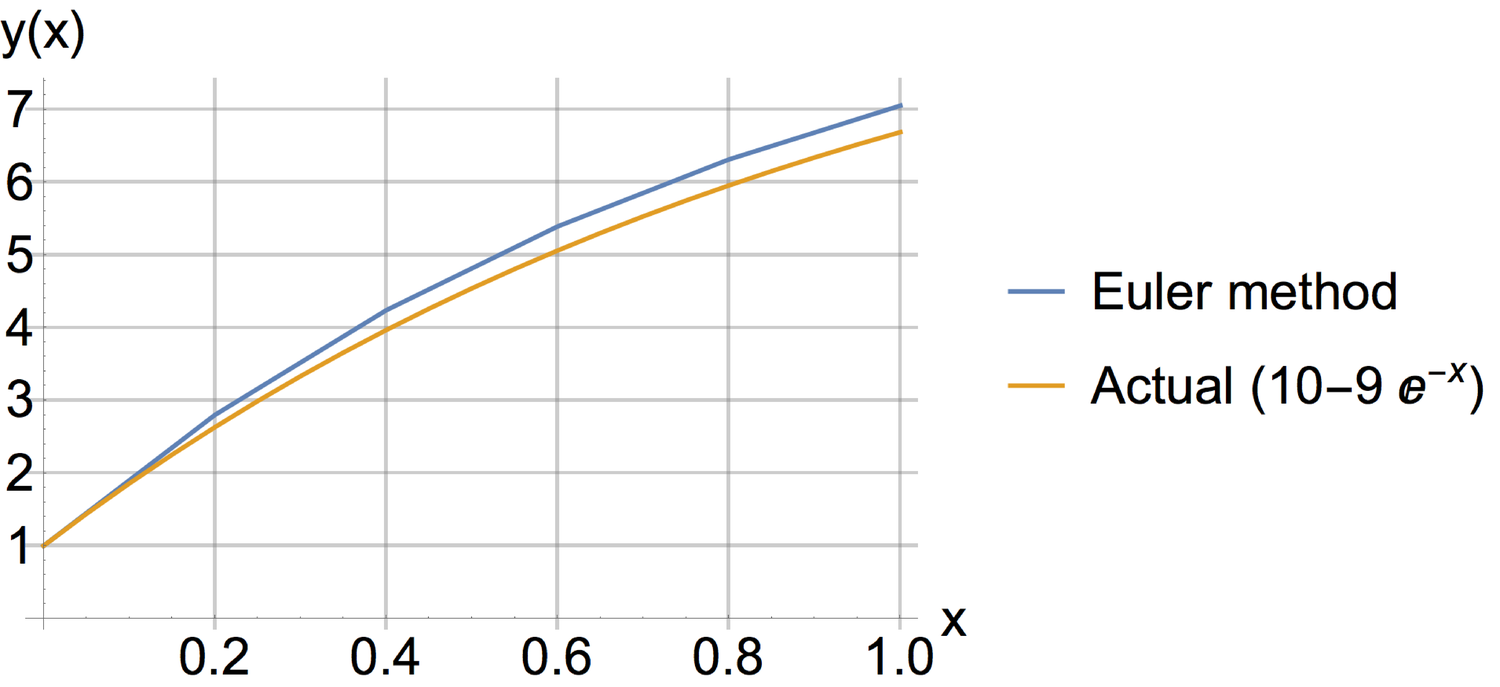
\includegraphics{eulers_method.png}

\subsection*{Solution}
\six{}

\hash{c}{1f90fa} 
% It would be nice to see if this error actually goes to zero in the end.




%%%%%%%%%%%%%%%%%%%%%%%%%%%%%%%%%
\newpage
%%%%%%%%%%%%%%%%%%%%%%%%%%%%%%%%%
\section{Exact differential equations: derivation}

\subsection*{Resources}
\begin{itemize}
    \item Videos: \url{https://www.khanacademy.org/math/differential-equations/first-order-differential-equations/exact-equations/v/exact-equations-intuition-1-proofy}
\end{itemize}

\subsection*{Challenge}
Please follow the two videos on derivation and intuition regarding exact differential equations starting at the video listed above.

If
\begin{equation}
    \frac{d \psi(x,y)}{dx} = 2xy + x^2y' - (x+y)/100
\end{equation}

what is $\displaystyle \frac{\partial \psi}{\partial x}$?

To check your answer, substitute $x=3.1$ and $y=-2$ into the resulting equation.

\subsection*{Solution}
\six{}

\hash{v}{f7f178}
% Note that video is not so clear about psi being a full rather than partial derivative. This question should help address this problem.




%%%%%%%%%%%%%%%%%%%%%%%%%%%%%%%%%
\newpage
%%%%%%%%%%%%%%%%%%%%%%%%%%%%%%%%%
\section{Exact differential equations: possible solutions given $\psi_x$}

\subsection*{Resources}
\begin{itemize}
    \item Videos: Exact equations intuition 1,2 and examples 1,2,3 starting from \url{https://www.khanacademy.org/math/differential-equations/first-order-differential-equations/exact-equations/v/exact-equations-intuition-1-proofy}
    \item Text: \url{http://tutorial.math.lamar.edu/Classes/DE/Exact.aspx}
\end{itemize}

\subsection*{Challenge}
Sum the points of all the possible solutions to the integral of the partial-differential equation:
\begin{equation}
    \psi_x = 6x - 3e^x sin(y)
\end{equation}

1 point: $\psi(x,y) = 3x^2-3e^x sin(y) + 4$

2 points: $\psi(x,y) = 3x^2-3e^x sin(y) + x$

4 points: $\psi(x,y) = 3x^2-3e^x sin(y) + y$

8 points: $\psi(x,y) = 3x^2-3e^x sin(y) + yx$

16 points: $\psi(x,y) = 3x^2-3e^x sin(y) + y^2$

32 points: $\psi(x,y) = 3x^2-3e^x sin(y) + 5 sin(y)$

64 points: $\psi(x,y) = 3x^2-3e^x sin(y) + 5 sin(y)cos(x)$

\subsection*{Solution}
\six{}

\hash{b}{408993} 




%%%%%%%%%%%%%%%%%%%%%%%%%%%%%%%%%
\newpage
%%%%%%%%%%%%%%%%%%%%%%%%%%%%%%%%%
\section{Exact differential equations: identification}
\label{sec:edeid}

\subsection*{Resources}
\begin{itemize}
    \item Videos: Exact equations intuition 1,2 starting from \url{https://www.khanacademy.org/math/differential-equations/first-order-differential-equations/exact-equations/v/exact-equations-intuition-1-proofy}
    \item Text: \url{http://tutorial.math.lamar.edu/Classes/DE/Exact.aspx}
\end{itemize}

\subsection*{Challenge}
Sum the points of the equations below that are exact differential equations:

1 point: $\displaystyle (3x^2y+8xy^2) dx + (x^3 + 8x^2y + 12 y^2) dy = 0$ % A

2 points: $\displaystyle sin(x) cos(y) dx + cos(x) sin(y) dy = 0$ % B

4 points: $\displaystyle sin(x) cos(y) dx + sin(x) sin(y) dy = 0$ % C

8 points: $\displaystyle \frac{dx}{x} + \frac{dy}{y} = 0$ % D

16 points: $\displaystyle -\frac{y dx + x dy}{x^2} = 0 $ % E

32 points: $\displaystyle -\frac{y dx - x dy}{x^2} = 0$ % F


\subsection*{Solution}
\six{}

\hash{n}{868f48} 




%%%%%%%%%%%%%%%%%%%%%%%%%%%%%%%%%
\newpage
%%%%%%%%%%%%%%%%%%%%%%%%%%%%%%%%%
\section{Exact differential equations: solving}

\subsection*{Resources}
\begin{itemize}
    \item Videos: Exact equations examples 1,2,3 starting from \url{https://www.khanacademy.org/math/differential-equations/first-order-differential-equations/exact-equations/v/exact-equations-example-1}
    \item Text: \url{http://tutorial.math.lamar.edu/Classes/DE/Exact.aspx}
\end{itemize}

\subsection*{Challenge}
In challenge \ref{sec:edeid} you should have identified 4 exact differential equations. Considering each of the 4 EDE's in order, try to solve the EDE's applying the following conditions:

\subsubsection{1st EDE}
Do not try to solve this one.

\subsubsection{2nd EDE}
Use the condition $y(\pi/4)=\pi/4$ to find an explicit solution for the equation and then evaluate $y$ at $x=\pi$.

\subsubsection{3rd EDE}
Use the condition $y(1)=3$ to find an explicit solution for the equation and then evaluate $y$ at $x=4$.

\subsubsection{4th EDE}
Use the condition $y(1)=2$ to find an explicit solution for the equation and then evaluate $y$ at $x=1$.


\subsection*{Solution}

\subsubsection{2nd EDE}
\six{}

\hash{m}{af87e2}

\subsubsection{3rd EDE}
\six{}

\hash{aa}{d01c3d}

\subsubsection{4th EDE}
\six{}

\hash{bb}{5e1074}




%%%%%%%%%%%%%%%%%%%%%%%%%%%%%%%%%
\newpage
%%%%%%%%%%%%%%%%%%%%%%%%%%%%%%%%%
\section{Exact differential equations: a useful integration method}

\subsection*{Challenge}
Obtain an expression for $g(x)$ in terms of $f(x)$ in the following integral:

\begin{equation}
    \int \frac{f'(x)}{f(x)} dx = g(x)
\end{equation}

ie, you should be able to re-write $g(x)$ in terms of a simple (non-integral) function of $f(x)$, in the form $g(x) = \cdots$.

\subsection*{Solution}
You can check your answer by putting a function of $x$ into $f(x)$.




%%%%%%%%%%%%%%%%%%%%%%%%%%%%%%%%%
\newpage
%%%%%%%%%%%%%%%%%%%%%%%%%%%%%%%%%
\section{Exact differential equations: integrating factors}
\label{sec:edeif}

\subsection*{Resources}
\begin{itemize}
    \item Videos: Integrating factors 1,2 starting from \url{https://www.khanacademy.org/math/differential-equations/first-order-differential-equations/exact-equations/v/integrating-factors-1}
\end{itemize}

\section*{Comment}
Note that in the videos, Sal Khan does an example considering an integrating factor of $\mu(x)$, but in some cases $\mu(y)$ leads to a solution more easily. You may need to try both to determine an answer.

\subsection*{Challenge}
Solve the exact differential equations below using integrating factors.

1. Solve the equation below using an integrating factor. Place the solution in the form $f(x,y) = C$, then calculate the value of $C$ when substituting $x=2$ and $y=1$ into the equation. Do not try to solve the equation to get it in the form $y(x)=\cdots$.

\begin{equation}
    \label{eq:edeif1}
    y dx + (2 x y - e^{-2 y}) dy = 0
\end{equation}

2. Calculate the integrating factor for the following equation. To check your answer, substitute $x=1$ or $y=1$ into any final expression, assuming an integration constant of zero.

\begin{equation}
    \label{eq:edeif2}
    y(3x-y) dx + x(x-y)dy = 0
\end{equation}

3. Show that $1/(x^y+y^2)$ is an integrating factor for the equation
\begin{equation}
    x dx + y dy + 4 y^3 (x^2 + y^2)dy = 0
\end{equation}

\subsection*{Solution}
Challenge related to equation \ref{eq:edeif1}: \hash{cc}{bb15d6}

Challenge related to equation \ref{eq:edeif2}: \hash{dd}{6a8742}




%%%%%%%%%%%%%%%%%%%%%%%%%%%%%%%%%
\newpage
%%%%%%%%%%%%%%%%%%%%%%%%%%%%%%%%%
\section{Exact differential equations: integrating factor derivation}
\label{sec:intfacderiv}

\subsection*{Challenge}
1. Starting from the equation

\begin{equation}
    \mu(x,y) M(x,y) dx + \mu(x,y) N(x,y) dy = 0
\end{equation}

show that if the integrating factor $\mu$ is only a function of $x$, then

\begin{equation}
    \label{eq:intfacmux}
    \mu_x = \mu \left ( \frac{M_y-N_x}{N} \right )
\end{equation}

2. Do the same, assuming that $\mu$ is only a function of $y$.

% NT do something for linear equations mu=e^\int(a)




%%%%%%%%%%%%%%%%%%%%%%%%%%%%%%%%%
\newpage
%%%%%%%%%%%%%%%%%%%%%%%%%%%%%%%%%
\section{Exact differential equations: integrating factor calculation}
\label{sec:edeifcalc}

\section*{Comment}
Without proof, we can use equation \ref{eq:intfacmux} to gain information about the existance of an integration factor. If $\left ( \frac{M_y-N_x}{N} \right )$ is a function of $x$ only, then we know that the integration factor is only a function of $x$, and it can be solved for by integration of equation \ref{eq:intfacmux}. The same can be said for $\mu(y)$ that you derived an expression for in challenge \ref{sec:intfacderiv}.

\subsection*{Challenge}
Use equations from section \ref{sec:intfacderiv} and information provided in the comment here to determine the integrating factor for

\begin{equation}
    \label{eq:edeifcalc1}
    e^x dx + (e^x Cot(y) + 2y Csc(y)) dy = 0
\end{equation}

and

\begin{equation}
    \label{eq:edeifcalc2}
    (x-y^2) dx + 2xy dy = 0
\end{equation}

To check your answer, for both cases substitute $x=\pi$ or $y=\pi$ into the integrating factor, and assume an integration constant of 1.

\subsection*{Solution}


Equation \ref{eq:edeifcalc1}: \hash{ee}{51a0ae}

Equation \ref{eq:edeifcalc2}: \hash{ff}{a56bce}




%%%%%%%%%%%%%%%%%%%%%%%%%%%%%%%%%
\newpage
%%%%%%%%%%%%%%%%%%%%%%%%%%%%%%%%%
\section{Summary of 1st-order differential equations}

\subsection*{Challenge}
1. Create a flowchart describing how you will approach solving a general 1st-order differential equation.

% Linear, Separable, Exact (with and without integration factors)
2. Solve the following 1st-order differential equations:

\begin{equation}
    \label{eq:1odegen1}
    y' - 4y = 8x + 3
\end{equation}
evaluated at $x=1$.

\begin{equation}
    \label{eq:1odegen2}
    4yy' = 8x + 3
\end{equation}
assuming an integration constant of zero and evaluating the final equation at $x=2$.

\begin{equation}
    \label{eq:1odegen3}
    y' + 4y = e^{-8x}
\end{equation}
assuming an integration constant of zero and evaluating the final equation at $x=1/8$.

\subsection*{Solution}
Equation \ref{eq:1odegen1}: \hash{qq}{a43ab2}

Equation \ref{eq:1odegen2}: \hash{rr}{990bfa}

Equation \ref{eq:1odegen3}: \hash{ss}{91989d}

\fi


% Benouli and substitution

% More advanced topics are in Paul's notes, but first check how much time is remaining.

% Do I need to add more challenges for simple 1st order linear equations?


\end{document}
